\section{Analysis and Discussion}
\label{sec:analysis}

\subsection{What Do Self-Supervised Encoders Learn?}
\label{sec:encoder_analysis}

A central question is \emph{why} different self-supervised objectives learn different representations, and how this explains their downstream performance.

\begin{table}[t]
\centering
\caption{Encoder representation quality. PC1 correlation measures how well the first principal component of the encoder's output aligns with RUL and the dominant degradation indicator (spectral centroid).}
\label{tab:encoder}
\small
\begin{tabular}{@{}lccc@{}}
\toprule
Metric & JEPA & Contrastive & Handcrafted \\
\midrule
PC1 correlation w/ RUL & 0.186 & \textbf{0.648} & 0.585 \\
PC1 correlation w/ spectral centroid & 0.071 & \textbf{0.856} & 1.000 \\
Max per-dim correlation w/ RUL & 0.144 & \textbf{0.648} & 0.585 \\
\bottomrule
\end{tabular}
\end{table}

\paragraph{JEPA learns waveform texture.} The JEPA objective - predicting masked patches from context - optimizes for local waveform reconstruction. The encoder must capture periodicity, amplitude modulation, and patch-level temporal structure. However, these features have low correlation with the spectral centroid (0.071), which is the primary degradation indicator for bearings. This explains why JEPA alone underperforms handcrafted spectral features for RUL prediction.

\paragraph{Contrastive learning captures degradation dynamics.} The temporal contrastive objective - distinguishing early from late snapshots - forces the encoder to learn what \emph{changes} over a bearing's life. The dominant change is spectral centroid shift (correlation 0.856 with PC1), which occurs as surface roughness increases and distributes vibrational energy across frequencies. This alignment with the degradation indicator explains the strong cross-dataset transfer: spectral centroid shift is a physics-invariant degradation signature.

\paragraph{Hybrid complementarity.} JEPA and contrastive representations are nearly orthogonal in their information content. JEPA captures fine-grained waveform features that are dataset-specific but informative within domain. Contrastive captures the slow, monotonic degradation trajectory that transfers across domains. The hybrid architecture leverages both, achieving the best overall performance.

\begin{figure}[t]
\centering
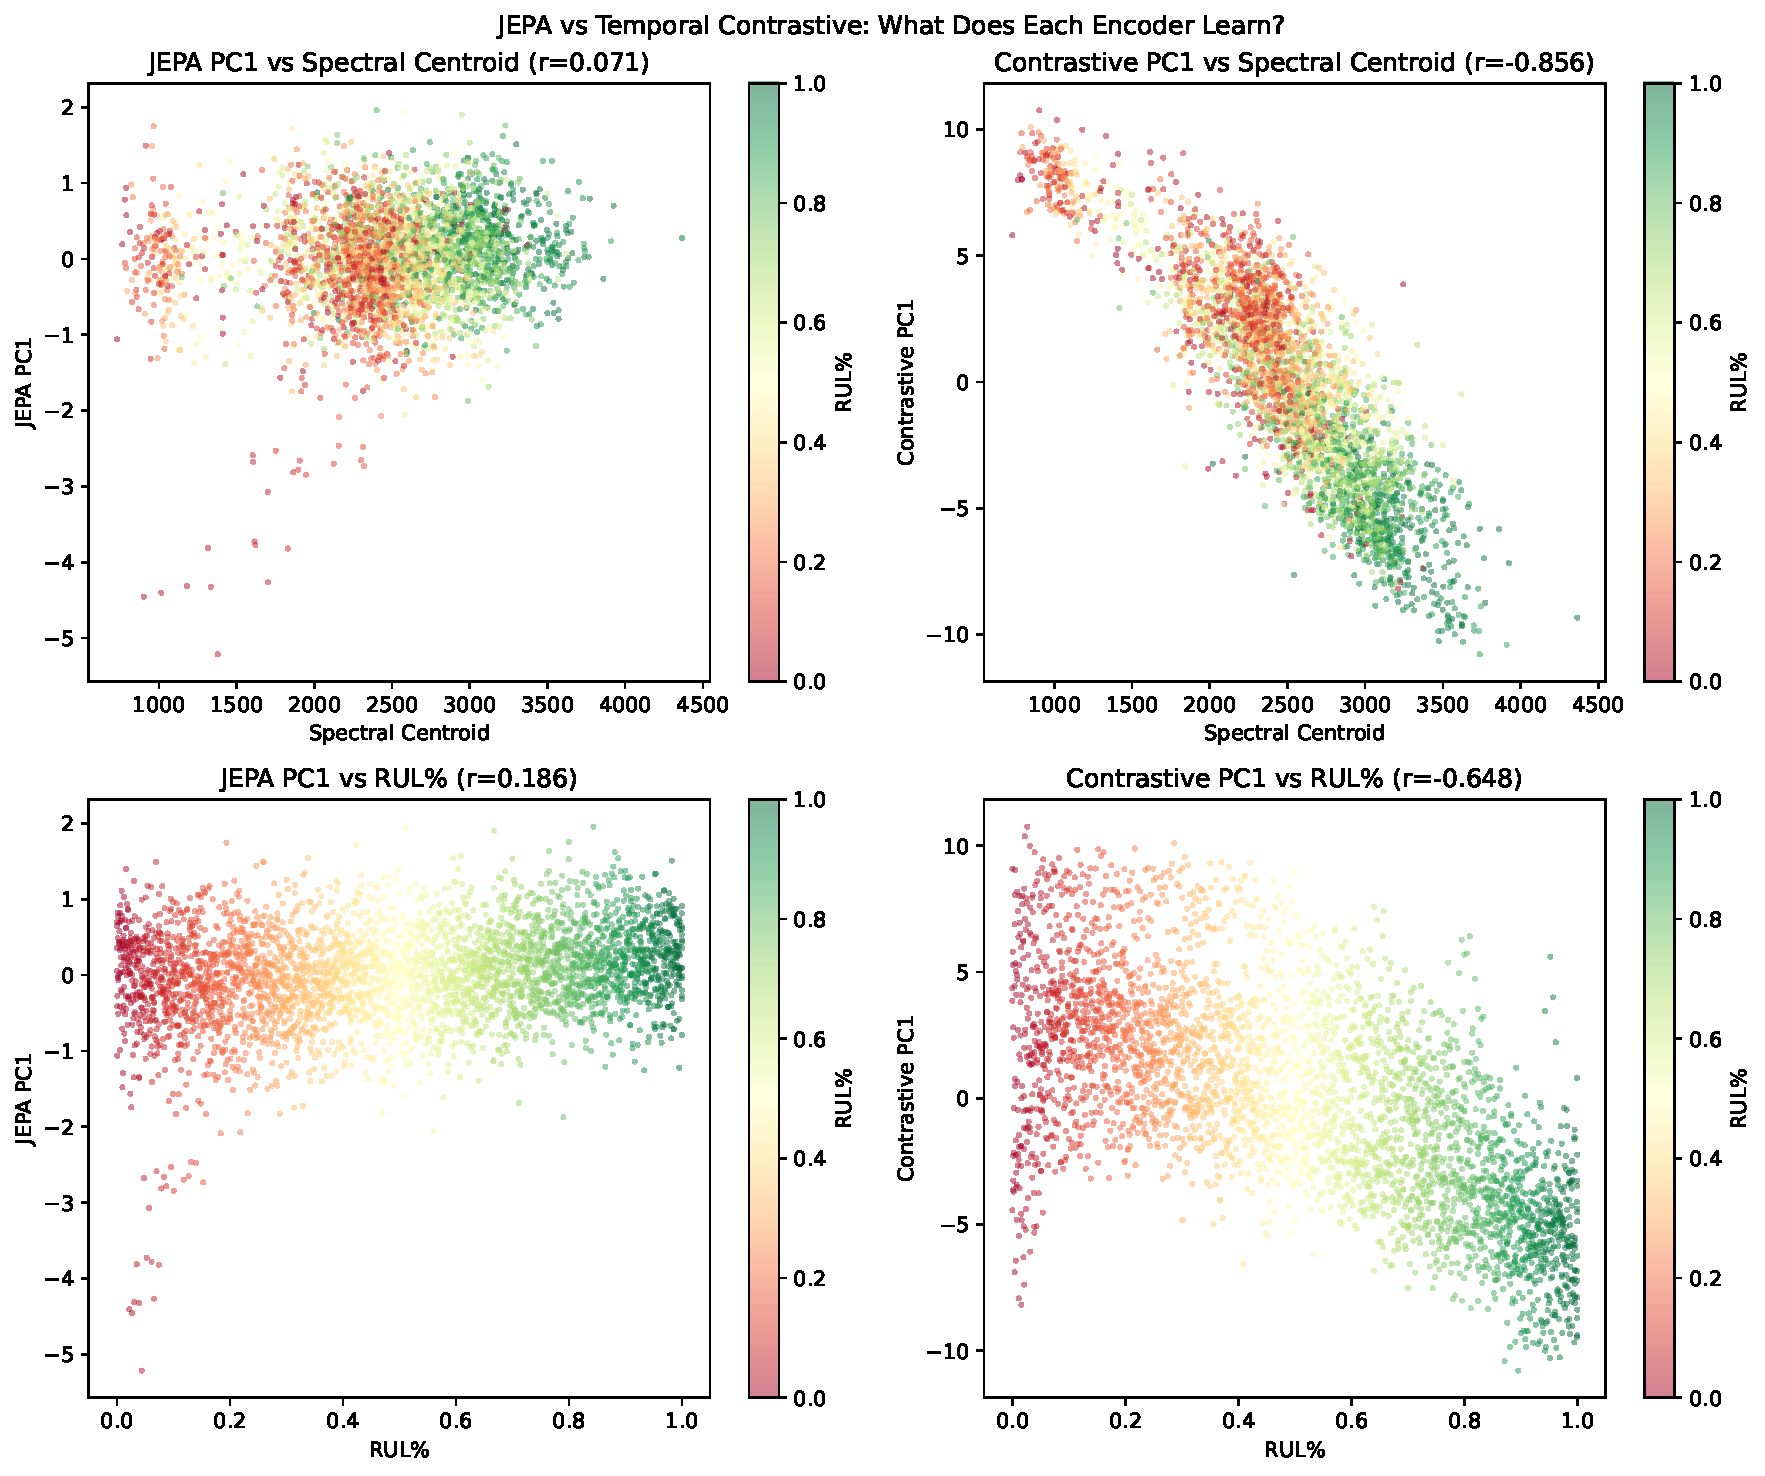
\includegraphics[width=\linewidth]{figures/v8_encoder_analysis.pdf}
\caption{PCA visualization of encoder representations. JEPA embeddings (left) show no clear degradation trajectory, while contrastive embeddings (center) align with spectral centroid shift. Handcrafted features (right) show the strongest monotonic trend.}
\label{fig:encoder_analysis}
\end{figure}

\begin{figure}[t]
\centering
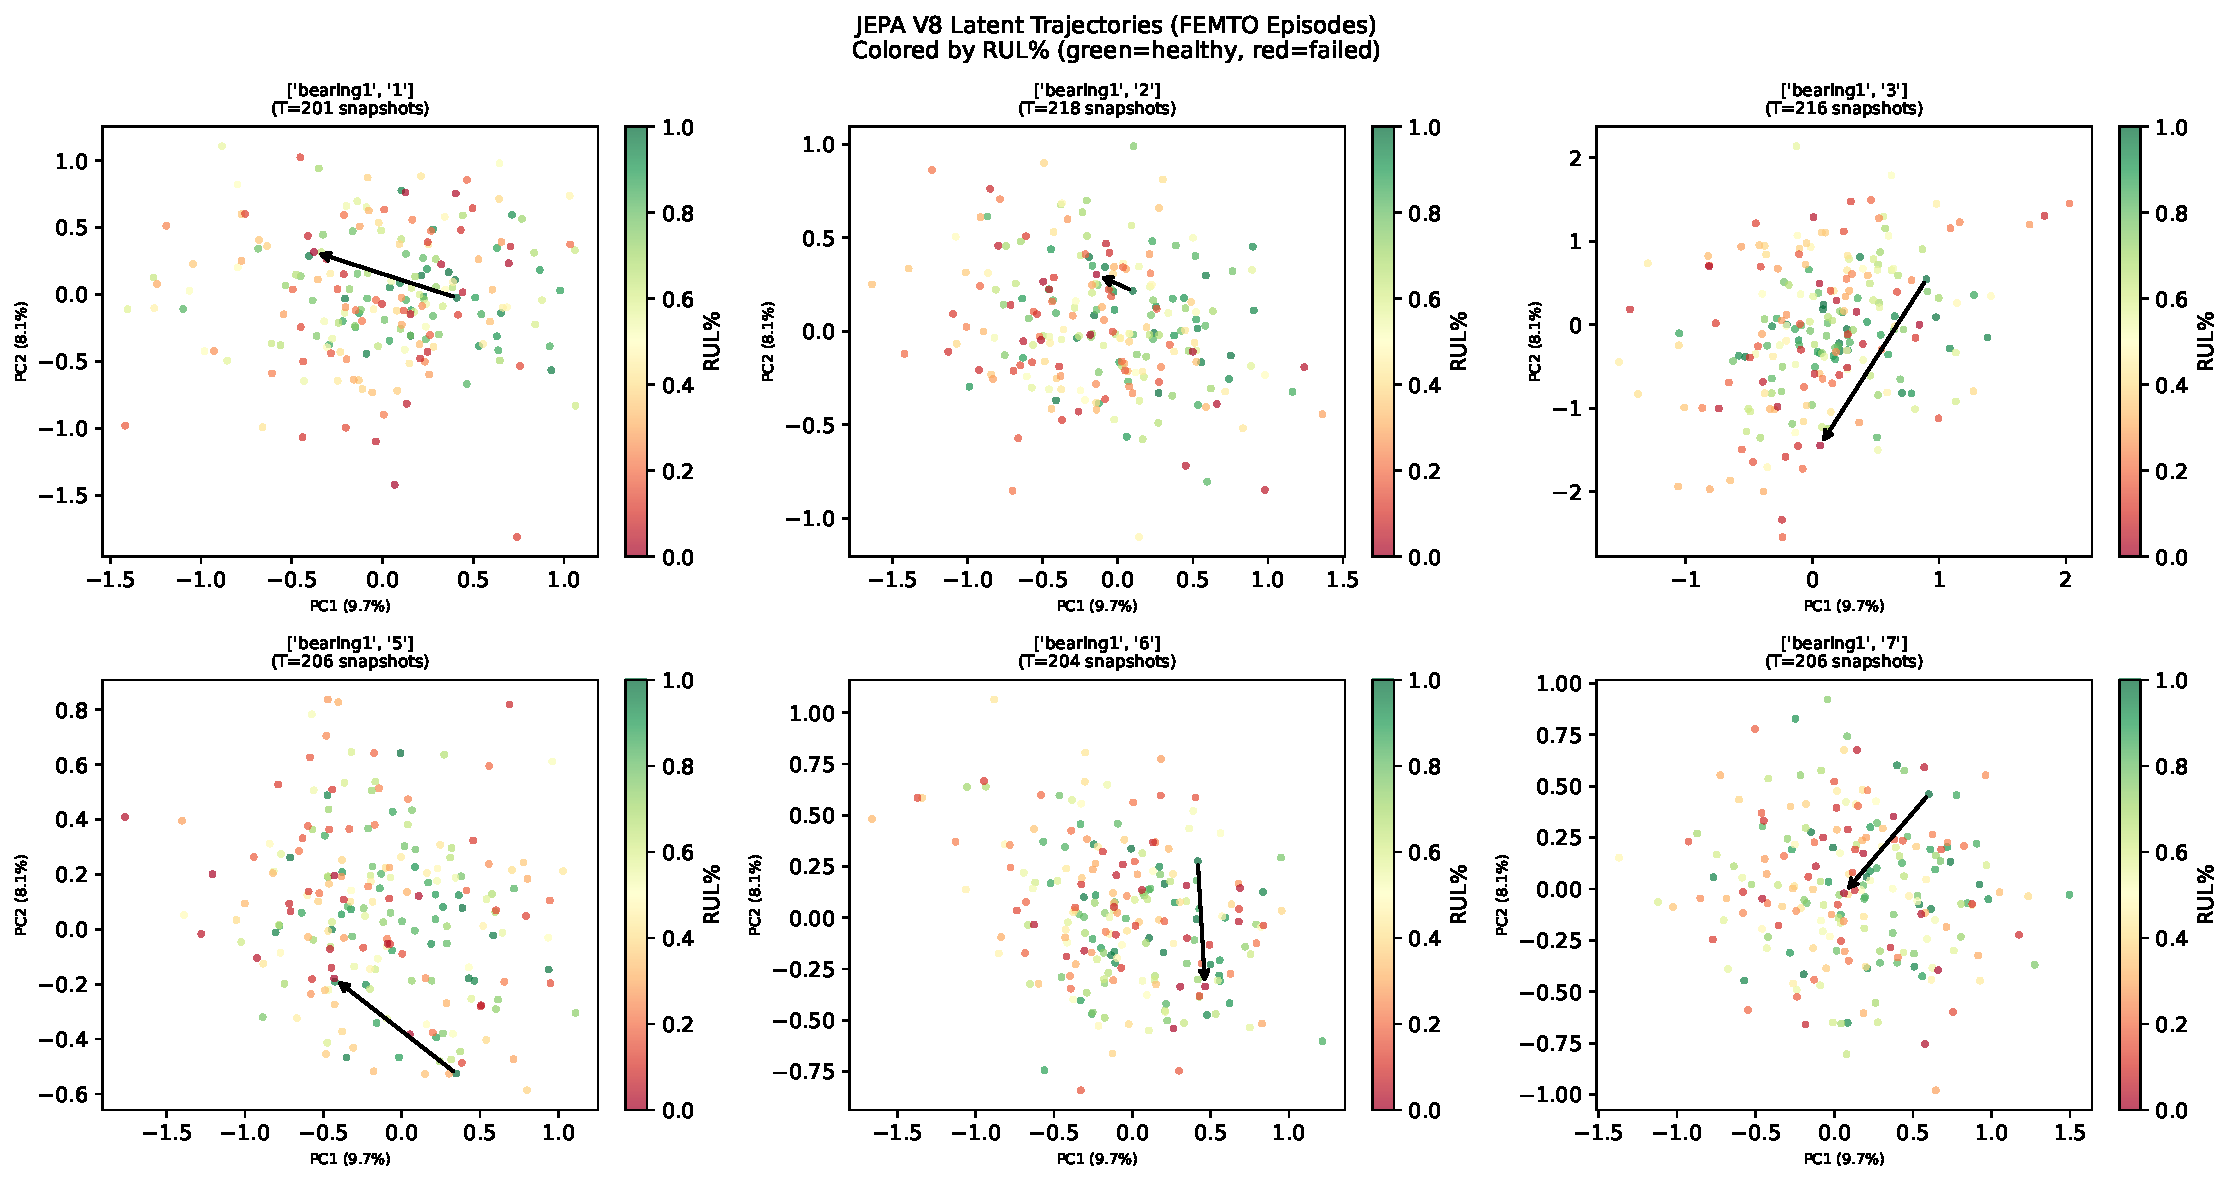
\includegraphics[width=\linewidth]{figures/v8_latent_trajectories.pdf}
\caption{Latent space trajectories over bearing lifetime. Each curve traces a single episode from healthy (start) to failure (end). Contrastive encoders produce smooth, monotonic trajectories aligned with degradation state.}
\label{fig:latent_trajectories}
\end{figure}

\subsection{When Does Transfer Succeed?}
\label{sec:transfer_analysis}

The divergent within-dataset vs.\ cross-dataset performance reveals a fundamental trade-off:

\begin{itemize}[nosep]
  \item \textbf{Within-dataset}: JEPA is preferred because fine-grained waveform features are discriminative when train/test distributions match. JEPA achieves RMSE 0.113 on FEMTO$\to$FEMTO vs.\ 0.142 for contrastive.
  \item \textbf{Cross-dataset}: Contrastive is preferred because only dataset-invariant features (spectral centroid shift) transfer. Contrastive achieves RMSE 0.227 on FEMTO$\to$XJTU vs.\ 0.280 for JEPA.
\end{itemize}

The coefficient of variation in episode lifetimes (CV = 0.635) explains why elapsed-time baselines fail cross-dataset: FEMTO bearings live 1--7 hours while XJTU-SY bearings live 0.5--2.6 hours, making calendar time a poor proxy for degradation state.

\subsection{Limitations}
\label{sec:limitations}

We identify several limitations of the current work:

\begin{enumerate}[nosep]
  \item \textbf{Small dataset.} With only 23 bearing episodes, our results have non-trivial variance (e.g., JEPA+LSTM std = 0.015). Each run-to-failure episode requires physically destroying a bearing, fundamentally limiting dataset scale.
  \item \textbf{Single channel.} Current experiments use only one vibration channel. Extending to multivariate sensor inputs is an important direction for future work.
  \item \textbf{Temporal contrastive requires episode structure.} The contrastive objective assumes access to run-to-failure episodes with temporal ordering. This is available in prognostics but not in all monitoring scenarios.
  \item \textbf{JEPA pretraining instability.} Training loss oscillates after epoch 2 on heterogeneous multi-source data; the best checkpoint is always early. This suggests the EMA dynamics interact poorly with high data heterogeneity.
  \item \textbf{Two transfer pairs.} Cross-dataset evaluation is limited to FEMTO$\leftrightarrow$XJTU-SY. Validation on additional domains (e.g., turbofan engines) would strengthen the generalization claims.
\end{enumerate}
